\section{Results}

\subsection{System}

All of the source code for this project is hosted in a GitHub repository.\footnote{https://github.com/juanyepesp/EyeNav} The repository holds the code for this documentation, the backend module, the chrome extension and the testing module.

\begin{figure}[ht]
    \centering
    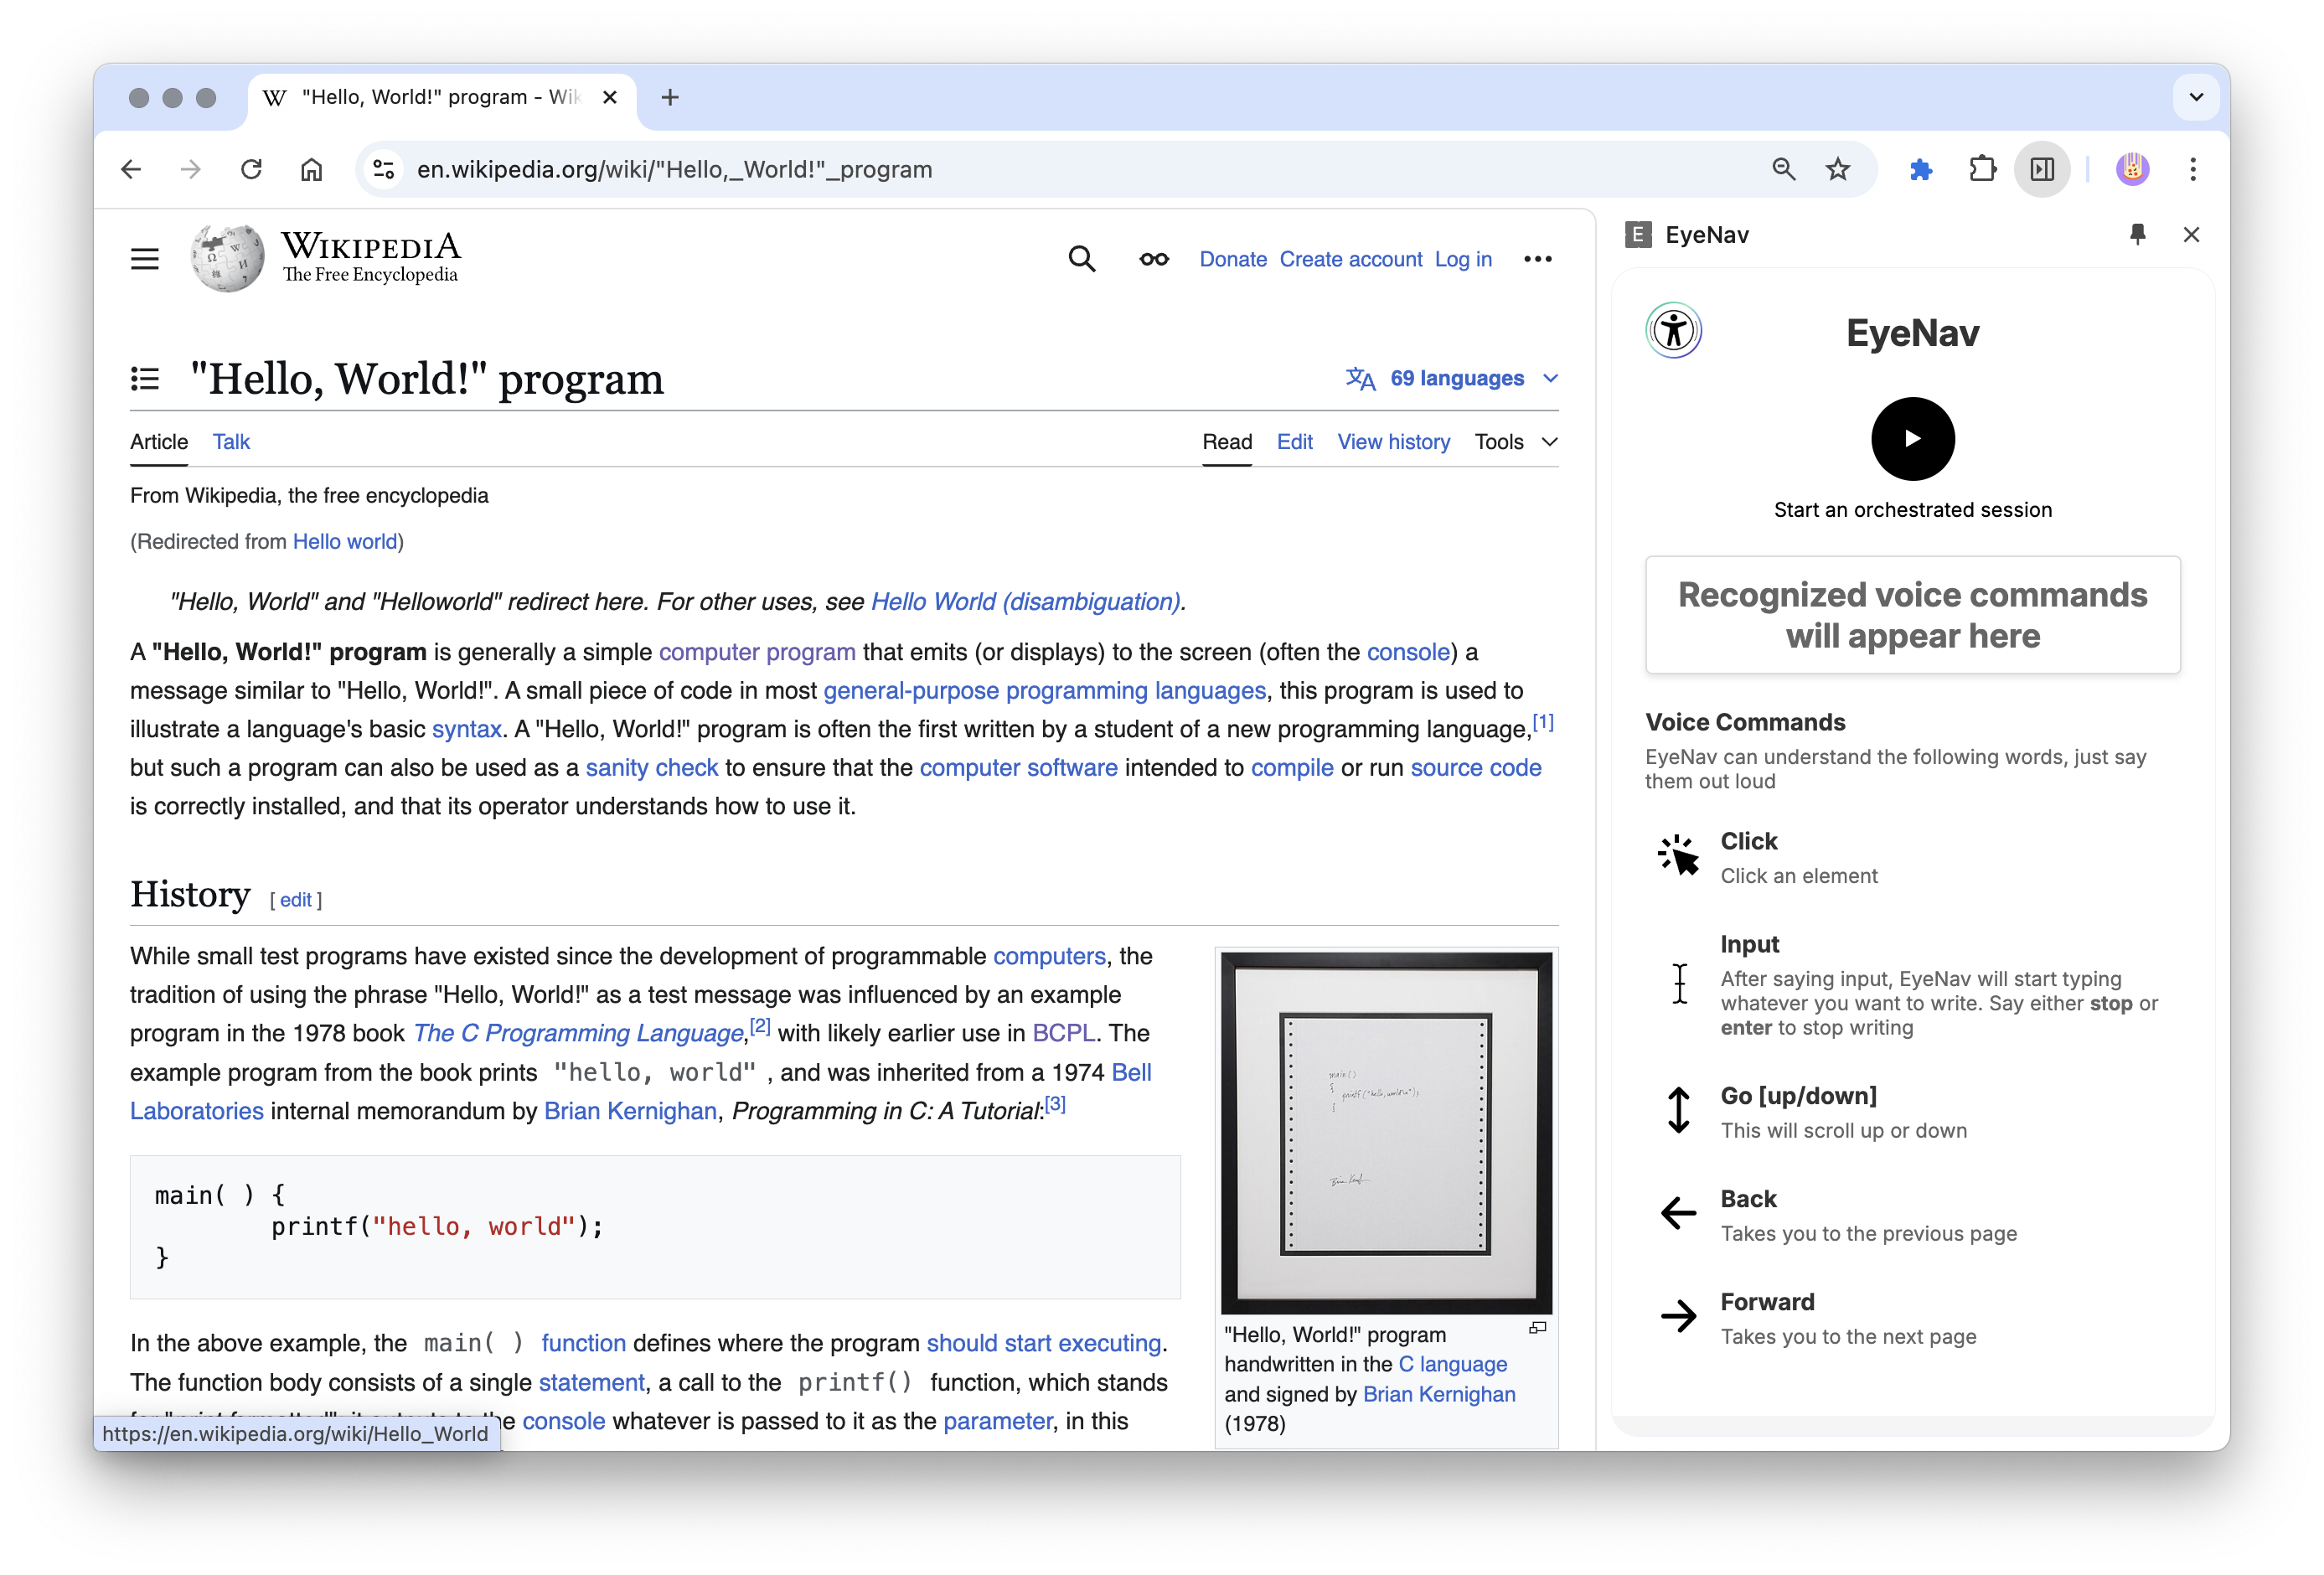
\includegraphics[width=1\textwidth]{images/screenshots/eyenav-1.png}
    \caption{First look of the extension working in Chrome}
    \label{fig:ss-1}
\end{figure}

\begin{figure*}[ht]
    \centering
    \begin{subfigure}[ht]{0.48\textwidth}
        \centering
        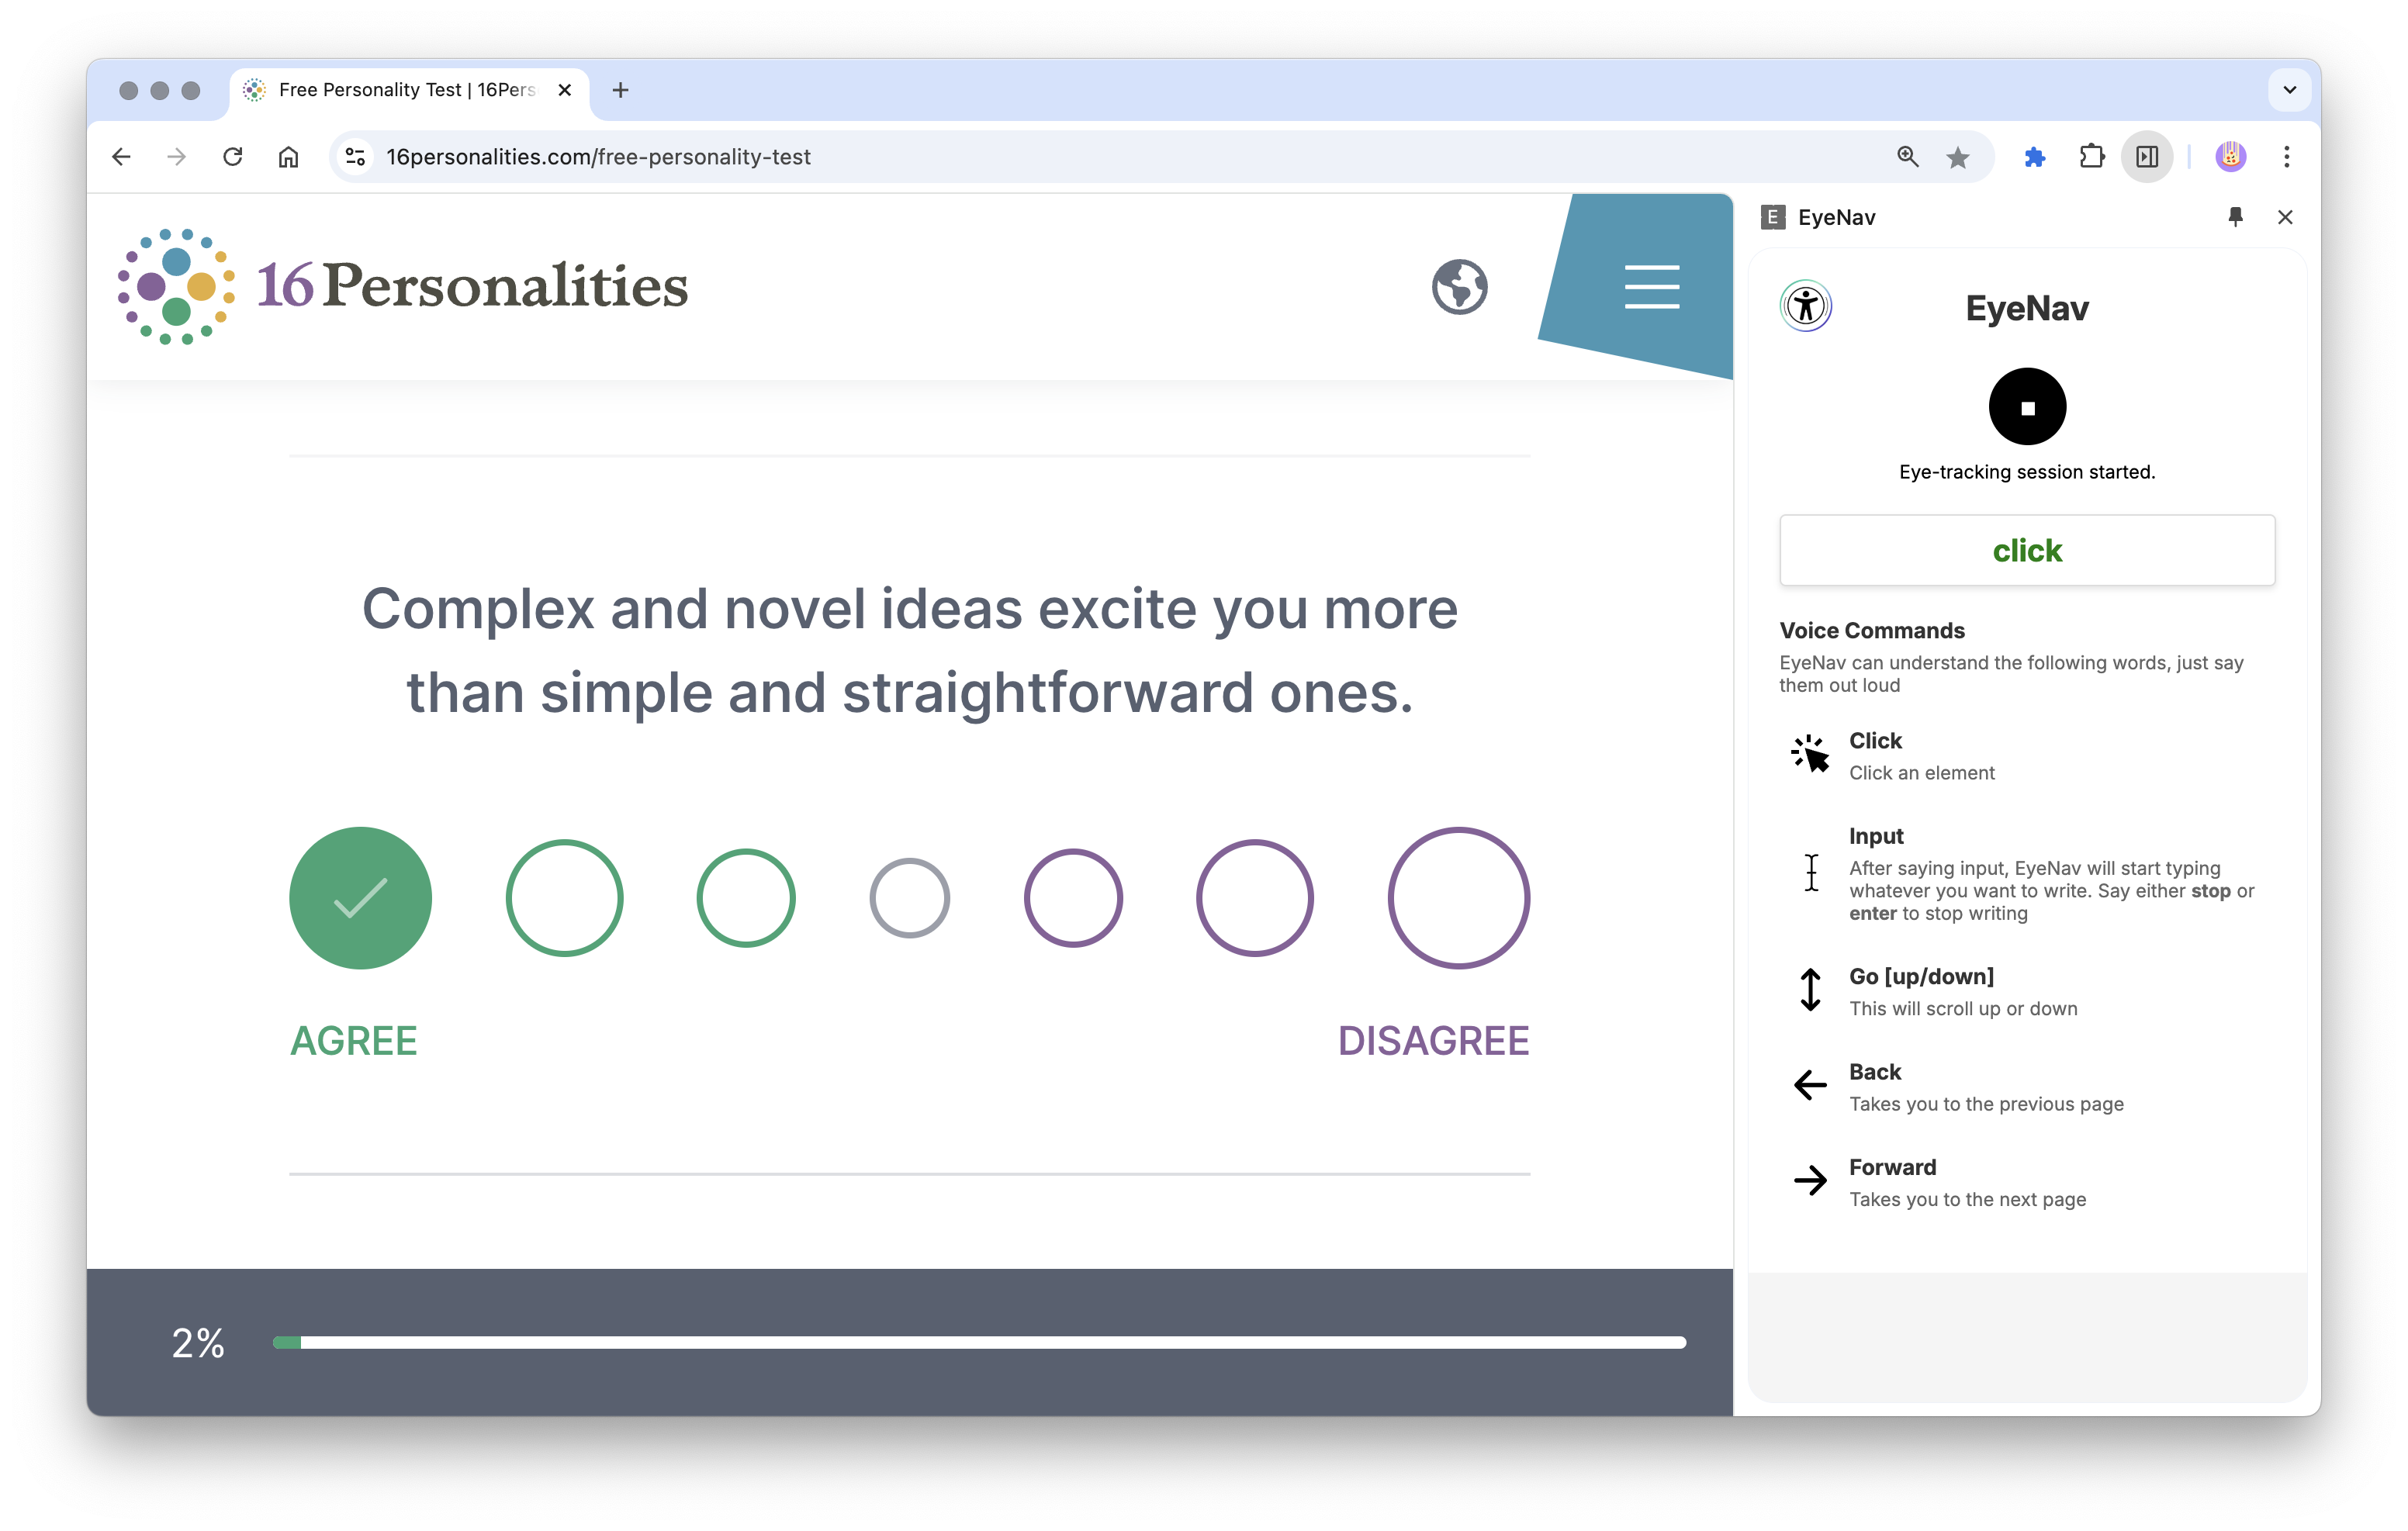
\includegraphics[width=\textwidth]{images/screenshots/eyenav-click.png}
        \caption{Clicking an item}
    \end{subfigure}%   
    ~ 
    \begin{subfigure}[ht]{0.48\textwidth}
        \centering
        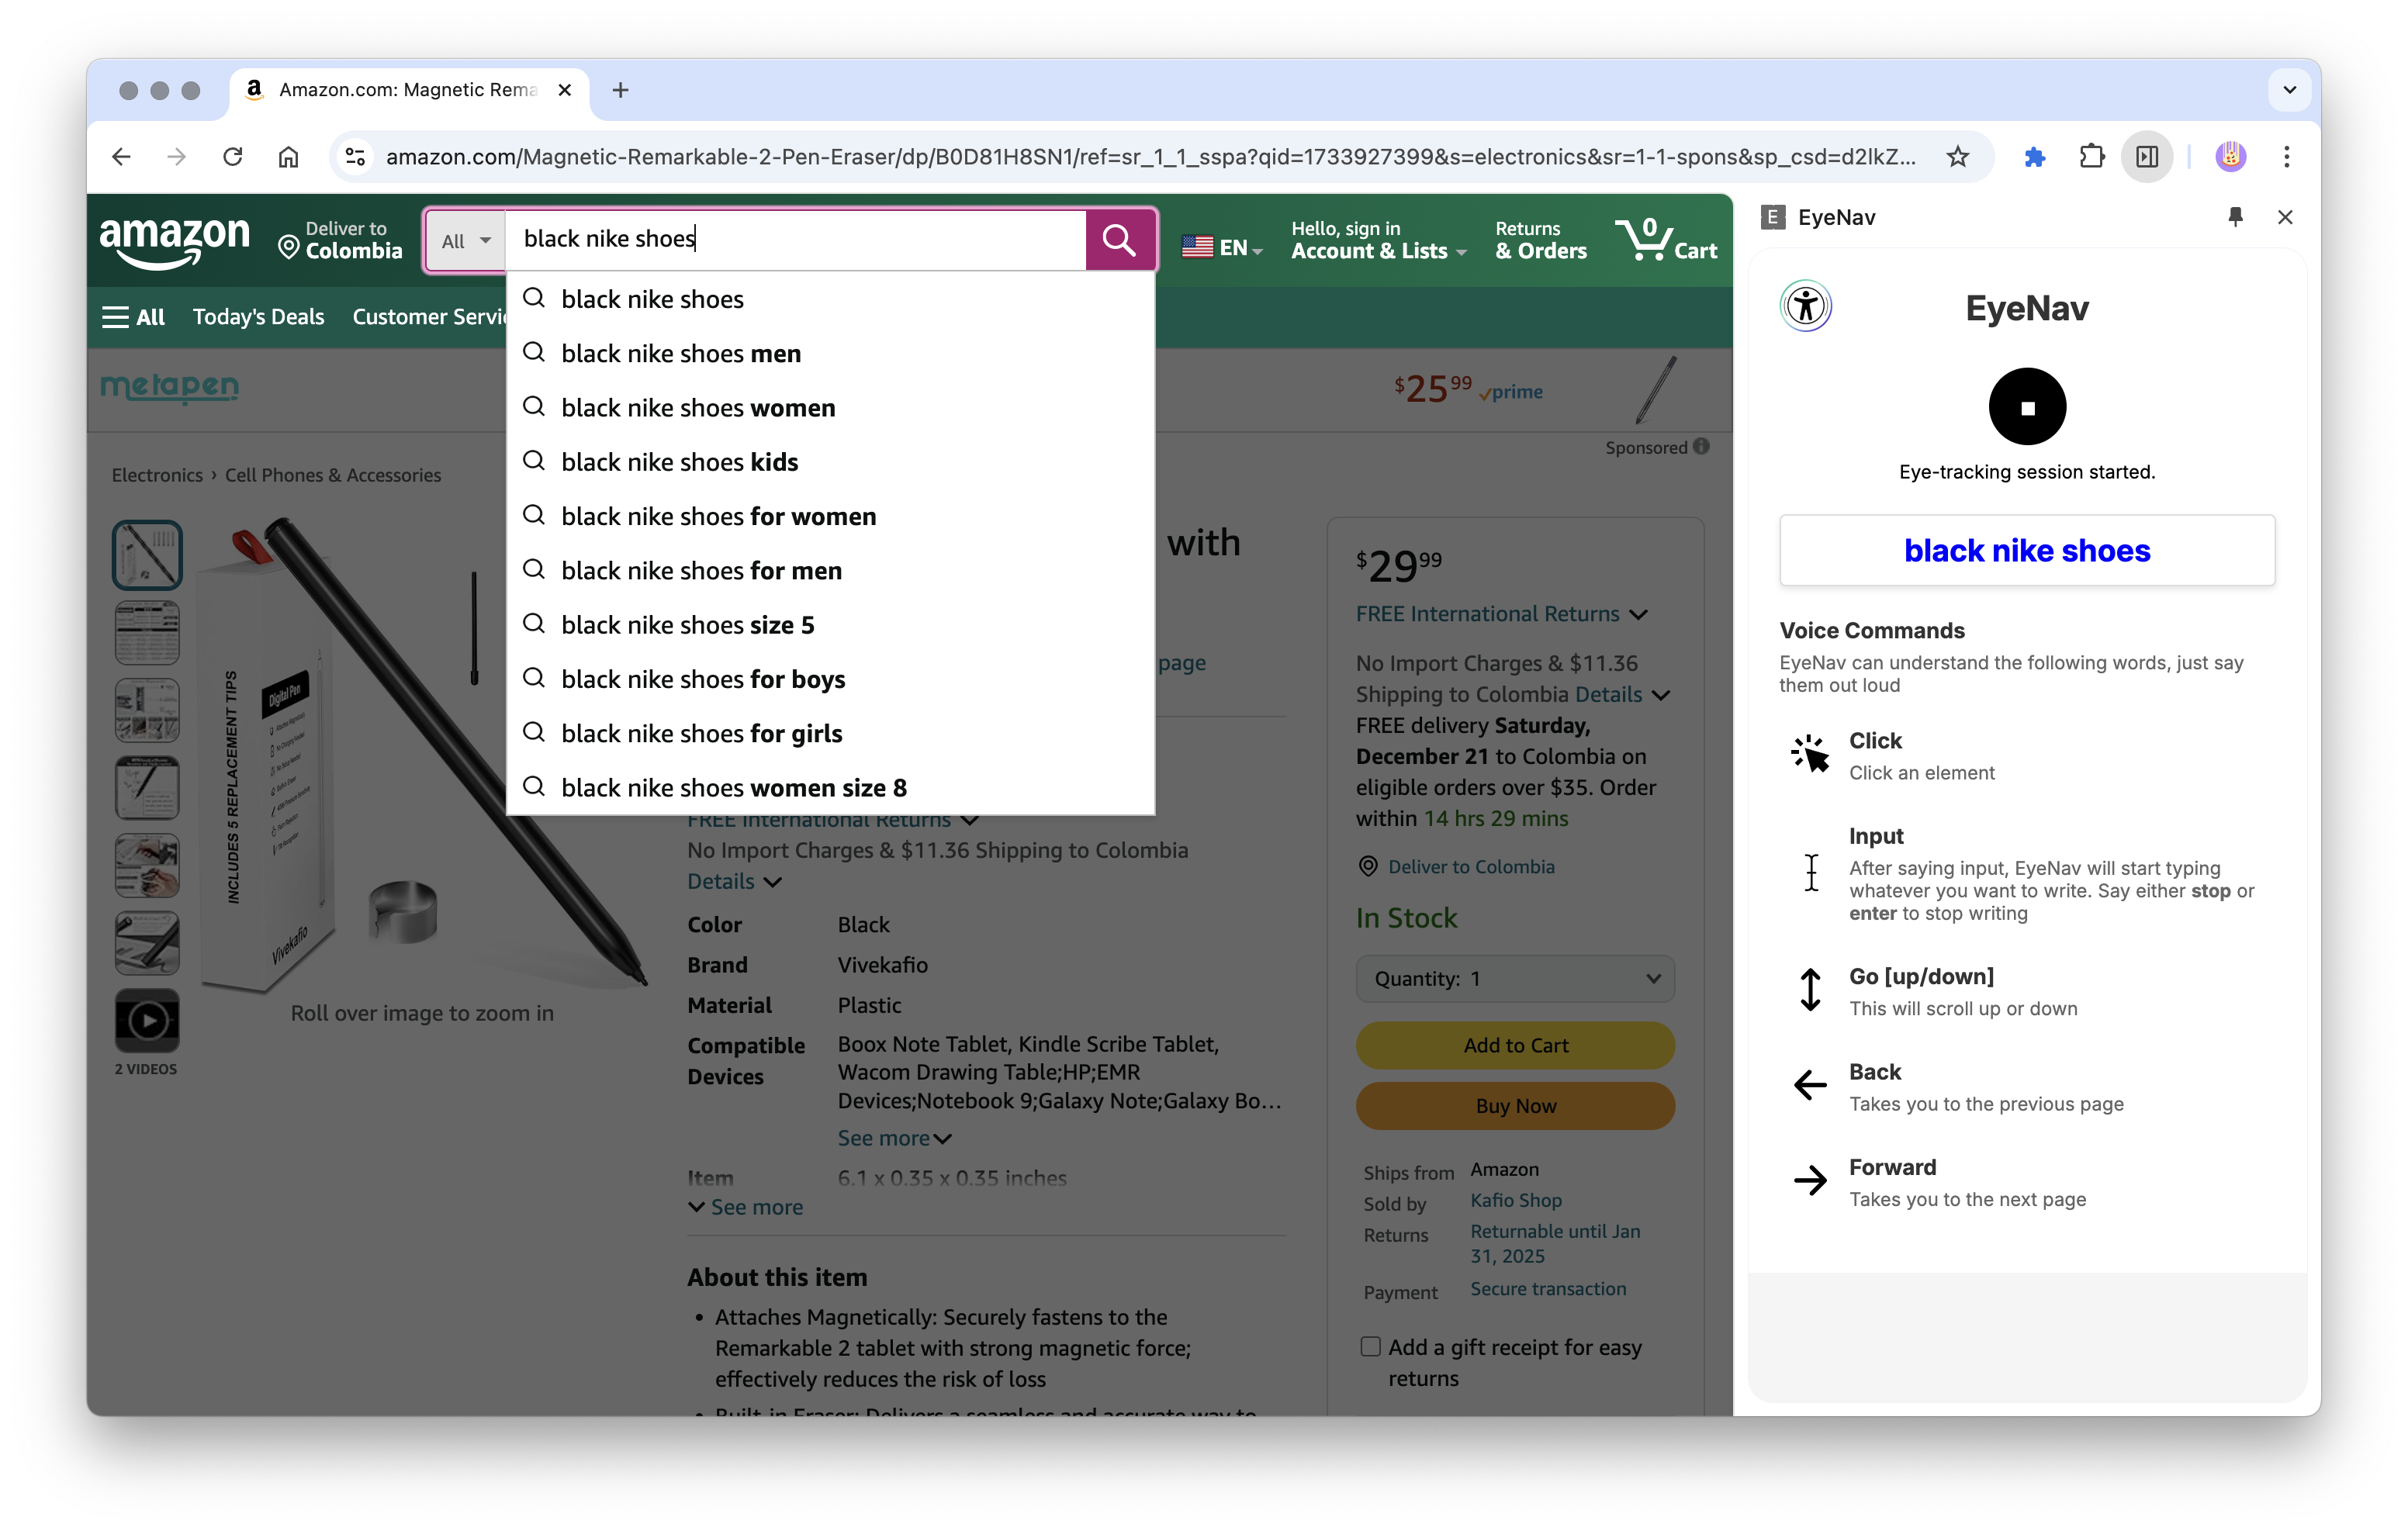
\includegraphics[width=\textwidth]{images/screenshots/eyenav-input.png}
        \caption{Inputting text}
    \end{subfigure}
    \caption{Other actions that can be done}
    \label{figs:ss-2-3}

\end{figure*}

Figures \ref{fig:ss-1} and \ref{figs:ss-2-3} display the system in action. 

\subsection{Usability}

Usability in itself is not an absolute metric, and needs to be defined in particular contexts where it is being applied. In that sense, ways of measuring this non-functional requirement are not straight-forward and do not depend on a single method, but are rather cualitative data that need to be analysed in this way.

\subsubsection{System Usabillity Scale}

The system usability scale (SUS) is useful for understanding broad and general measurements of usability. Proposed by \cite{art:sus-1996}, this scale is widely used in systems engineering, and consists of 10 questions that the user will assess subjectively, but ultimately can point out how the system in three points:

\begin{itemize}
    \item effectiveness (the ability of users to complete tasks using the system, and the quality of the output of those tasks)
    \item efficiency ( the level of resource consumed in performing tasks)
    \item satisfaction (users subjective reactions to using the system). \citep{art:sus-1996}
\end{itemize}

These are the statements proposed in the scale, where the subject can mark from 1 (strongly disagree) to 5 (strongly agree):

\begin{enumerate}[label=\textbf{\arabic*.}]
    \item I would like to use this system frequently. \hfill \underline{1 \quad 2 \quad 3 \quad 4 \quad 5}
    \item I found the system unnecessarily complex. \hfill \underline{1 \quad 2 \quad 3 \quad 4 \quad 5}
    \item I thought the system was easy to use. \hfill \underline{1 \quad 2 \quad 3 \quad 4 \quad 5}
    \item I think I would need technical support to use this system. \hfill \underline{1 \quad 2 \quad 3 \quad 4 \quad 5}
    \item The functions of the system were well integrated. \hfill \underline{1 \quad 2 \quad 3 \quad 4 \quad 5}
    \item There was too much inconsistency in the system. \hfill \underline{1 \quad 2 \quad 3 \quad 4 \quad 5}
    \item Most people would learn to use this system very quickly. \hfill \underline{1 \quad 2 \quad 3 \quad 4 \quad 5}
    \item I found the system very cumbersome to use. \hfill \underline{1 \quad 2 \quad 3 \quad 4 \quad 5}
    \item I felt very confident using the system. \hfill \underline{1 \quad 2 \quad 3 \quad 4 \quad 5}
    \item I needed to learn a lot of things before I could get going with this system. \hfill \underline{1 \quad 2 \quad 3 \quad 4 \quad 5}
\end{enumerate}

SUS have scores ranging from 0 to 100. Each individual score can be calculated like formula \ref{eq:sus} shows, where each $s_n$ represents each statement

\begin{equation}
    2.5 \left(20 \sum(s_1,s_3,s_5,s_7,s_9) - \sum(s_2,s_4,s_6,s_8,s_{10})\right) \label{eq:sus}
\end{equation}

Furthermore, in the usability tests conducted, the average SUS was \verb|76.7|, with the highest score being \verb|95| and the lowest \verb|55|. Indicating that the system was found to be quite usable.


\subsubsection{Interviews}

% TODO poner los comentarios de las entrevistas

\subsection{Accesibility}

According to the \cite{techreport:webaim-2024}, \verb|95.9%| of webpages have at least one detectable accessibility error.


% TODO poner los comentarios de las entrevistas

\subsection{Test Scripts Generation}

The tests that the system performs are a set of actions that were recorded when the user was using the system. These actions are written as steps in Gherkin syntax, which are then interpreted and each one corresponds to a Webdriver action the s=testing module can replay. An example test is shown.

\begin{lstlisting}
    Feature: Replay of session on Nov 19 at 02:10:49 PM

    @user1 @web
    Scenario: User interacts with the web page named "Wikipedia, the free encyclopedia"
    
        Given I navigate to page "https://en.wikipedia.org/wiki/Main_Page"
        And I click on tag with selector a with href "/wiki/Samantha_Harvey_(author)"
        And I click on tag with selector a with href "/wiki/Ditton,_Kent"
        And I click on tag with selector "input" with id "searchInput"
        And I input "hello world"
        And I click on tag with selector a with href "https://en.wikipedia.org/w/index.php?title=Special%3ASearch&search=%22Hello%2C+World%21%22+program&wprov=acrw1_0"
        And I click on tag with selector a with href "/wiki/Computer_program"
        And I go back
        And I scroll down
\end{lstlisting}
